\documentclass[11pt]{article}

\usepackage[margin=1in]{geometry}
\usepackage{amsmath,amssymb,amsthm}
\usepackage{booktabs}
\usepackage{graphicx}
\usepackage{url}
\usepackage[hidelinks]{hyperref}

\newtheorem{proposition}{Proposition}
\newtheorem{remark}{Remark}

\title{\bfseries Clustered Safety Events and the Effective Sample Size\\
in Autonomous Vehicle Fleet Rate Estimation}

\author{Pouria Emami Tabrizi}

\date{September 2026}

\begin{document}
\maketitle

\begin{abstract}
Autonomous vehicle fleet validation estimates rare-event rates --- safety-relevant
disengagements, near-misses, contact events --- per mile driven, and attaches
confidence statements to those estimates. The estimators in current use treat
logged events as independent arrivals of a Poisson process. Real fleet events are
not independent: a construction zone, a rain hour, or a single poorly handled
intersection produces several correlated events. We model the event stream as a
compound Poisson (Neyman--Scott) process and show that ignoring this clustering
inflates the variance of the rate estimator by a design effect
$D = E[K^2]/E[K]$, where $K$ is the cluster size. Three consequences follow. First,
a nominal $95\%$ confidence interval has asymptotic coverage
$2\Phi(z_{0.975}/\sqrt{D}) - 1$, which falls to $74\%$ at $D=3$ and $54\%$ at
$D=7$. Second, the mileage required to demonstrate that a fleet's event rate lies
below a safety target is understated by exactly the factor $D$, which suggests
that standard mileage calculations may understate the evidence required. Third,
empirical-Bayes shrinkage weights of the form $n/(n+k)$ over-weight noisy local
estimates, costing up to $7.8\times$ in mean squared error in our study. We give
a correction that substitutes an effective sample size $n_{\text{eff}} = n/\hat{D}$,
where $\hat{D}$ is estimated from the logs themselves, and show by simulation
that it restores nominal coverage across the range studied. We then measure
$\hat{D}$ on public California DMV autonomous vehicle disengagement reports.
Pooled across fleets it is $4.79$ for 2023 and $5.29$ for 2024, and per-fleet
estimates range from $1.00$ to $13.77$ --- so the design effect is neither
negligible nor a constant that can be assumed. As a negative control we repeat
the measurement on NHTSA Standing General Order driverless incident reports,
where the vehicle-day design effect is $1.02$: the estimator returns unity when
events genuinely do not recur on the clustering unit, which both supports the
larger values and scopes the correction to the event classes that do recur.
\textbf{The simulation study uses synthetic data. The measured design effects
come from regulatory filings, and the two sources describe different event
classes --- safety-driver disengagements and driverless reportable incidents ---
which is the distinction the negative control turns on.} This is an independent
preprint and has not been peer reviewed.
\end{abstract}

\section{Introduction}

The central statistical difficulty of autonomous vehicle (AV) safety validation is
that the events of interest are rare. Kalra and Paddock~\cite{kalra2016driving}
showed that demonstrating a fatality rate lower than the human benchmark with
reasonable confidence would require hundreds of millions of miles, a result that
has shaped a decade of subsequent work. Liu and Feng~\cite{liu2024curse} give the
modern statement of the problem as a ``curse of rarity'': the information content
per mile is so low that direct estimation is impractical without variance
reduction, and much recent effort has gone into importance sampling and
scenario-based testing to recover statistical power.

Much of this work rests on a modelling assumption that is seldom made explicit
and, as far as we are aware, not yet examined directly: that the safety-relevant
events logged by a fleet are \emph{independent}. Terres et al.~\cite{terres2023behavioral} model the count
of behavioral events over $m$ miles as $\mathrm{Poisson}(\theta m)$, which embeds
independence in the likelihood. Chen et al.~\cite{chen2026confidence} assume
i.i.d.\ features and a Poisson sample size in deriving confidence intervals for
importance-sampled rate estimates; the authors note explicitly that ``how to
properly design the run segments to minimize spatial-temporal dependencies is
beyond the scope of the current paper.'' Zhao et al.~\cite{zhao2025need}, in a
paper arguing for exactly the statistical rigour we are concerned with here,
adopt i.i.d.\ Bernoulli scenario models while acknowledging that the simplification
``may not hold due to factors like software updating of the AV or changing
environments.''

The independence assumption is analytically convenient and in many settings
harmless. In this one, we argue, it is unlikely to hold, in a specific and
consequential way. Safety-relevant events arrive in clusters. A
construction zone that the perception stack handles poorly produces several
disengagements in a few minutes. A rain hour degrades detection across an entire
shift. One unprotected left turn geometry generates the same near-miss on every
pass. The clusters are not a nuisance detail of the logging pipeline; they are how
the underlying failure modes express themselves.

This paper makes the consequence precise. We model the event stream as a compound
Poisson process, derive the resulting variance inflation, and quantify what it
costs. The contribution is deliberately narrow:

\begin{enumerate}
\item We show that the naive Poisson rate estimator remains unbiased but that its
variance is inflated by a design effect $D = E[K^2]/E[K]$
(Section~\ref{sec:formulation}).
\item We give the exact asymptotic coverage of the naive confidence interval as a
function of $D$, and confirm it by simulation (Proposition~\ref{prop:coverage}).
\item We show that the mileage required to demonstrate a safety target scales
linearly in $D$ (Proposition~\ref{prop:miles}), which is the safety-critical
consequence: a fleet using the standard calculation concludes ``demonstrated''
before the evidence supports it.
\item We give a correction based on an effective sample size that is estimable
from fields fleets already log, and show it restores nominal coverage
(Sections~\ref{sec:correction} and~\ref{sec:simulation}).
\item We measure $\hat{D}$ on public California DMV disengagement filings for
2023 and 2024, covering twelve fleets, and find pooled values near $5$ with
per-fleet values spanning $1.00$ to $13.77$ (Section~\ref{sec:practice}).
\item We repeat the measurement on NHTSA driverless incident reports as a
negative control, obtain $\hat{D} = 1.02$ at the vehicle-day, and use it to scope
the claim (Section~\ref{sec:negcontrol}).
\end{enumerate}

We are explicit about what this is not. The design effect is textbook survey
statistics~\cite{kish1965survey,cochran1977sampling}, and cluster-robust variance
estimation is standard~\cite{liang1986longitudinal}. No new mathematics is claimed.
The contribution is to connect that machinery to a setting where it has not yet
been applied, to quantify what its absence costs in the regime AV validation
operates in, and to note that the correction requires no new instrumentation.

\section{Related Work}

\paragraph{Fleet-level rate estimation.} The line of work most directly affected is
the estimation of event rates from fleet logs. Terres et
al.~\cite{terres2023behavioral} develop maximum likelihood procedures for rate
estimation under partial event review, using a Poisson model for the event count.
Chen et al.~\cite{chen2026confidence} construct confidence intervals for
importance-sampled rate estimates, assuming independent features. Zhao et
al.~\cite{zhao2025need} propose a probability-of-failure-per-scenario metric and
i.i.d.\ Bernoulli models for scenario-based testing. None of these addresses
clustering, serial dependence, or effective sample size directly. Two of the three
are explicit that dependence lies outside their scope, and it is that explicitness
which makes the present extension straightforward to state.

\paragraph{Traffic conflict extremes.} A separate and considerably more
dependence-aware literature estimates crash risk from traffic conflicts using
extreme value theory, beginning with Songchitruksa and
Tarko~\cite{songchitruksa2006extreme}. Zheng and Sayed~\cite{zheng2019bayesian}
develop non-stationary Bayesian hierarchical peak-over-threshold models, and more
recent work in the same literature extends conditional peak-over-threshold models
with self- and cross-exciting structure and with spatio-temporal hierarchies.
This machinery explicitly models dependence between extreme observations.

It does not, however, transfer directly to the fleet setting, and the reason
matters for the present paper. Self-exciting and conditional peak-over-threshold
models describe a single, densely observed excitation stream at one site: an
intersection under continuous video observation, where every conflict is recorded
and the excitation kernel is identifiable from inter-event times. Fleet validation
aggregates sparse events across many routes, operating conditions, and software
releases, where the dependence is \emph{nested} --- an event sits within a scene,
within a drive, within a release --- rather than generated by one excitation
process in one time series. Nested dependence of this kind is what design effects
and cluster-robust variance estimators are built for, and a point-process
excitation model is not the natural description of it.

\paragraph{Dependence corrections elsewhere.} Extreme value theory has long handled
dependent exceedances by declustering, with the extremal index quantifying the
degree of clustering~\cite{ferro2003inference}. In survey statistics the design
effect~\cite{kish1965survey,cochran1977sampling} plays the same role for clustered
sampling designs, and generalized estimating
equations~\cite{liang1986longitudinal} provide cluster-robust variance estimates
for correlated observations. In financial machine learning, López de
Prado~\cite{lopezdeprado2018advances} identifies overlapping event labels as a
source of inflated effective sample size and proposes average-uniqueness weighting
and sequential bootstrapping as remedies. The present paper connects these adjacent
treatments to the fleet rate estimation setting, where the same difficulty arises
but the corresponding corrections have not yet been carried over.

\section{Problem Formulation}
\label{sec:formulation}

\subsection{A clustered event process}

Let a fleet accumulate $m$ miles. We model safety-relevant events as a compound
Poisson process of Neyman--Scott type~\cite{neyman1958statistical}. Let cluster
centres --- distinct difficult contexts, such as one construction zone encountered
once, one rain hour, one problematic intersection geometry --- arrive as a Poisson
process with rate $\lambda_c$ per mile, so that the number of clusters is
$N_c \sim \mathrm{Poisson}(\lambda_c m)$. Each cluster $i$ contributes $K_i$
logged events, with $K_1, K_2, \dots$ independent and identically distributed on
$\{1, 2, \dots\}$, independent of $N_c$. The total event count is
\begin{equation}
N = \sum_{i=1}^{N_c} K_i .
\end{equation}
The quantity validation cares about is the event rate per mile,
\begin{equation}
\theta = \lambda_c \, E[K],
\end{equation}
estimated by $\hat{\theta} = N/m$. The classical Poisson model is the special case
$K \equiv 1$.

\subsection{The design effect}

By the standard compound Poisson moment identities,
\begin{equation}
E[N] = \lambda_c m \, E[K],
\qquad
\mathrm{Var}(N) = \lambda_c m \, E[K^2].
\end{equation}
The estimator $\hat{\theta} = N/m$ is therefore unbiased for $\theta$, with
\begin{equation}
\mathrm{Var}(\hat{\theta})
= \frac{\lambda_c E[K^2]}{m}
= \frac{\theta}{m} \cdot \frac{E[K^2]}{E[K]}
= \frac{\theta D}{m},
\qquad
D := \frac{E[K^2]}{E[K]} .
\label{eq:deff}
\end{equation}
We call $D$ the design effect, by analogy with clustered survey
sampling~\cite{kish1965survey}. It satisfies $D \geq 1$, with equality if and only
if every cluster has size one. Writing $\mu_K = E[K]$, an equivalent form is
$D = \mu_K + \mathrm{Var}(K)/\mu_K$: clustering hurts both through the mean cluster
size and through its dispersion.

An analyst who assumes independence uses $\mathrm{Var}(\hat\theta) = \theta/m$ and
therefore understates the standard error by a factor of $\sqrt{D}$. Note that the
point estimate is unaffected. The damage is entirely to the uncertainty
statement --- which, in a safety argument, is the part that carries the claim.

\begin{remark}
Equation~\eqref{eq:deff} is the perfectly-correlated case of Kish's design
effect $D = 1 + (\bar{K} - 1)\rho$, corresponding to $\rho = 1$: every event in a
cluster is treated as carrying the information of the same underlying failure
mode. A process with partial within-cluster correlation interpolates between
$D = 1$ and the value in~\eqref{eq:deff}, so the figures reported here should be
read as the design effect implied by whatever clustering the analyst's own logs
exhibit, not as a universal constant.
\end{remark}

\subsection{Coverage of the naive interval}

\begin{proposition}[Undercoverage]
\label{prop:coverage}
Let $\hat{\theta} = N/m$ and let the naive interval be
$\hat{\theta} \pm z_{1-\alpha/2}\sqrt{\hat{\theta}/m}$. As $m \to \infty$ with
$\theta$ and $D$ fixed, the asymptotic coverage of this interval is
\begin{equation}
2\,\Phi\!\left(\frac{z_{1-\alpha/2}}{\sqrt{D}}\right) - 1 ,
\end{equation}
where $\Phi$ is the standard normal distribution function.
\end{proposition}

\begin{proof}
By the central limit theorem for compound Poisson sums,
$(\hat{\theta} - \theta)\sqrt{m/(\theta D)} \Rightarrow \mathcal{N}(0,1)$. The
naive half-width is $z_{1-\alpha/2}\sqrt{\hat\theta/m}$, and
$\hat\theta \to \theta$ in probability, so the half-width is asymptotically
$z_{1-\alpha/2}\sqrt{\theta/m}$, which equals $z_{1-\alpha/2}/\sqrt{D}$ true
standard errors. Coverage is therefore the probability that a standard normal
variate lies within $z_{1-\alpha/2}/\sqrt{D}$ of zero.
\end{proof}

For a nominal $95\%$ interval this gives $87.1\%$ at $D = 1.67$, $74.2\%$ at
$D = 3$, and $54.1\%$ at $D = 7$. At the upper end of that range the interval's
actual coverage bears little relation to its nominal level.

\subsection{Miles required to demonstrate a target}

Validation programmes are usually framed as a demonstration: show, with
confidence $1 - \alpha$, that the fleet's event rate lies below some target
$\theta^{*} > \theta$. Using the upper confidence limit
$\hat\theta + z_{1-\alpha/2}\sqrt{\mathrm{Var}(\hat\theta)}$ and
solving for the mileage at which it falls below $\theta^{*}$ gives the following.

\begin{proposition}[Required mileage]
\label{prop:miles}
Under the clustered process, the mileage required for the upper confidence limit
to fall below $\theta^{*}$ is
\begin{equation}
m_{\text{req}} = \frac{z_{1-\alpha/2}^{2} \, \theta \, D}{(\theta^{*} - \theta)^{2}},
\end{equation}
which exceeds the mileage computed under the independence assumption by exactly a
factor of $D$.
\end{proposition}

This is the statement with the most direct practical consequence. For design
effects in the range studied here, a programme that sizes its mileage under the
independence assumption and stops at that figure will have accumulated between one
third and one seventh of the evidence implied by its own confidence statement. We
note that the discrepancy runs in the less cautious direction.

\section{Proposed Correction}
\label{sec:correction}

The correction is to estimate $D$ from the logs and use it. Suppose the $N$ logged
events can be partitioned into $C$ observed clusters with sizes
$K_1, \dots, K_C$. A natural moment estimator of the design effect is
\begin{equation}
\hat{D} = \frac{\sum_{i=1}^{C} K_i^{2}}{\sum_{i=1}^{C} K_i},
\label{eq:dhat}
\end{equation}
which is the sample analogue of $E[K^2]/E[K]$. The effective sample size is then
\begin{equation}
n_{\text{eff}} = \frac{N}{\hat{D}},
\end{equation}
and the corrected interval is
\begin{equation}
\hat{\theta} \pm z_{1-\alpha/2}\,\frac{\sqrt{N \hat{D}}}{m}
= \hat{\theta} \pm z_{1-\alpha/2}\,\frac{\sqrt{N}}{m}\sqrt{\hat{D}} .
\end{equation}
The required-mileage formula of Proposition~\ref{prop:miles} is corrected by the
same factor.

\paragraph{Shrinkage weights.} The same substitution repairs a second estimator.
Sparse per-segment or per-scenario rates are commonly stabilised by shrinking them
toward a fleet-level prior with an empirical-Bayes weight $w = n/(n+k)$, so that a
segment with few events leans on the prior and a segment with many events leans on
its own data. Under clustering, $n$ overstates the independent information
available, $w$ is therefore too large, and the estimator leans on a noisier local
estimate than the evidence supports. Substituting
$w_{\text{eff}} = n_{\text{eff}}/(n_{\text{eff}} + k)$ restores the intended
behaviour. This is the same defect López de Prado~\cite{lopezdeprado2018advances}
identifies for overlapping labels in financial machine learning, arriving here by a
different route.

\paragraph{What counts as a cluster.} The estimator~\eqref{eq:dhat} requires that
cluster membership be observable. In fleet logging it usually is, at least
approximately, because every logged event already carries identifiers that induce a
natural grouping: the vehicle and the calendar date, the drive or run segment, the
scene or map location, the weather condition, or the software release. Any of these
defines a partition; the appropriate choice is the one matching the failure mode
under study. We return to this in Section~\ref{sec:practice}.

\section{Simulation Study}
\label{sec:simulation}

\paragraph{Setup.} We simulate the process of Section~\ref{sec:formulation} with a
true rate of $\theta = 10^{-4}$ events per mile (one per ten thousand miles) over
a $5{,}000{,}000$ mile deployment, with $20{,}000$ replications per configuration.
Cluster sizes are drawn from a geometric distribution on $\{1,2,\dots\}$ with
parameter $p$, giving mean cluster size $1/p$ and design effect $D = (2-p)/p$. All
data are synthetic; the accompanying script \texttt{sim\_clustered\_av\_rates.py}
reproduces every figure reported here.

\paragraph{Coverage.} Table~\ref{tab:coverage} reports the actual coverage of a
nominal $95\%$ interval. The simulated coverage of the naive interval agrees with
Proposition~\ref{prop:coverage} to within one percentage point throughout, and the
corrected interval holds its nominal level across the whole range.
Figure~\ref{fig:coverage} shows the same result over a finer grid.

\begin{table}[htbp]
\centering
\caption{Actual coverage of a nominal $95\%$ confidence interval for the fleet
event rate. Synthetic data; $20{,}000$ replications per row.}
\label{tab:coverage}
\begin{tabular}{rrrrrr}
\toprule
Mean cluster size & $D$ & Naive (sim.) & Naive (theory) & Corrected & CI width ratio \\
\midrule
1.00 & 1.00 & 94.8\% & 95.0\% & 94.8\% & 1.00$\times$ \\
1.33 & 1.67 & 86.9\% & 87.1\% & 94.9\% & 1.29$\times$ \\
2.00 & 3.00 & 73.2\% & 74.2\% & 94.5\% & 1.73$\times$ \\
2.86 & 4.71 & 63.0\% & 63.3\% & 94.4\% & 2.17$\times$ \\
4.00 & 7.00 & 53.6\% & 54.1\% & 94.6\% & 2.64$\times$ \\
\bottomrule
\end{tabular}
\end{table}

\begin{figure}[htbp]
\centering
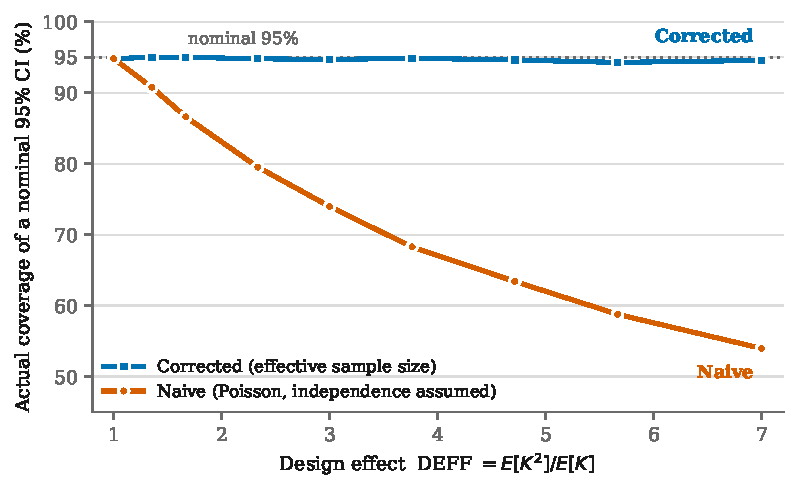
\includegraphics[width=0.8\textwidth]{coverage_vs_deff.pdf}
\caption{Actual coverage of a nominal $95\%$ confidence interval as a function of
the design effect. The naive interval degrades steadily; the effective-sample-size
correction holds the nominal level. Synthetic data.}
\label{fig:coverage}
\end{figure}

A mean cluster size of $2$ --- two logged events per difficult context, which is
not an extreme value for fleet data --- already reduces a nominal $95\%$
interval to $73\%$ actual coverage.

\paragraph{Required mileage.} Table~\ref{tab:miles} reports the mileage needed for
the upper confidence limit to fall below a target of $1.5\theta$. The ratio is
exactly $D$, as Proposition~\ref{prop:miles} requires.

\begin{table}[htbp]
\centering
\caption{Mileage required to demonstrate that the event rate lies below
$\theta^{*} = 1.5\theta$ at $95\%$ confidence, with $\theta = 10^{-4}$ per mile.}
\label{tab:miles}
\begin{tabular}{rrrrr}
\toprule
Mean cluster size & $D$ & Assuming independence & Corrected & Shortfall \\
\midrule
1.00 & 1.00 & 153,658 & 153,658 & 1.00$\times$ \\
1.33 & 1.67 & 153,658 & 256,097 & 1.67$\times$ \\
2.00 & 3.00 & 153,658 & 460,975 & 3.00$\times$ \\
2.86 & 4.71 & 153,658 & 724,389 & 4.71$\times$ \\
4.00 & 7.00 & 153,658 & 1,075,608 & 7.00$\times$ \\
\bottomrule
\end{tabular}
\end{table}

\paragraph{Shrinkage.} Table~\ref{tab:shrinkage} reports the mean squared error of
a per-segment rate blended toward an unbiased fleet-level prior with $k = 15$, over
$200{,}000$ miles. Because the prior is unbiased by construction, the entire gap is
variance: using the nominal event count costs up to $7.8\times$ in mean squared
error relative to using the effective count.

\begin{table}[htbp]
\centering
\caption{Mean squared error of an empirical-Bayes blended per-segment rate,
using the nominal event count $n$ versus the effective count
$n_{\text{eff}} = n/\hat{D}$, with $k = 15$.}
\label{tab:shrinkage}
\begin{tabular}{rrrrr}
\toprule
Mean cluster size & $D$ & MSE, nominal $n$ & MSE, effective $n$ & Ratio \\
\midrule
1.00 & 1.00 & $1.647 \times 10^{-10}$ & $1.647 \times 10^{-10}$ & 1.00$\times$ \\
1.33 & 1.67 & $2.766 \times 10^{-10}$ & $1.757 \times 10^{-10}$ & 1.57$\times$ \\
2.00 & 3.00 & $5.172 \times 10^{-10}$ & $1.785 \times 10^{-10}$ & 2.90$\times$ \\
2.86 & 4.71 & $8.658 \times 10^{-10}$ & $1.774 \times 10^{-10}$ & 4.88$\times$ \\
4.00 & 7.00 & $1.292 \times 10^{-9}$  & $1.655 \times 10^{-10}$ & 7.81$\times$ \\
\bottomrule
\end{tabular}
\end{table}

\section{Design Effects Measured on Public Fleet Data}
\label{sec:practice}

Nothing in Section~\ref{sec:correction} requires new instrumentation, and this is
the practical argument for the correction: $\hat{D}$ is computable from records
that already exist, including public ones.

\paragraph{California DMV disengagement reports.} Manufacturers testing autonomous
vehicles on California public roads file annual disengagement
reports~\cite{cadmv_disengagement}. The published CSV files contain one row per
disengagement, with fields for the manufacturer, the date, the vehicle
identification number, whether a driver was present, what initiated the
disengagement, the road type, and a free-text description of the cause. The date
and vehicle identifier together define a vehicle-day, which is a natural and
conservative cluster unit: events logged by the same vehicle on the same day are
candidates for sharing an underlying context.

\subsection{Measured design effects}

We computed~\eqref{eq:dhat} over vehicle-day clusters for the 2023 and 2024
testing-with-a-driver filings, retaining fleets with at least $30$ reported
events in a year. This covers $6{,}562$ events across $2{,}989$ vehicle-days in
2023 and $1{,}773$ events across $981$ vehicle-days in 2024. Rows with blank
manufacturer, date, or vehicle identifier were excluded; in both files every
such row was entirely empty, an artefact of the export, so no reported event was
discarded. Results are in Table~\ref{tab:empirical}.

\begin{table}[htbp]
\centering
\caption{Design effects estimated from California DMV disengagement reports,
using the vehicle-day as the cluster unit. Fleets with fewer than $30$ reported
events in a year are shown as ``--''. These are safety-driver disengagements,
not driverless safety events; see the caveats below.}
\label{tab:empirical}
\begin{tabular}{lrrrr}
\toprule
& \multicolumn{2}{c}{2023} & \multicolumn{2}{c}{2024} \\
\cmidrule(lr){2-3}\cmidrule(lr){4-5}
Fleet & Events & $\hat{D}$ & Events & $\hat{D}$ \\
\midrule
Apple & 3,194 & 3.44 & 285 & 1.60 \\
Ghost Autonomy & 1,034 & 7.73 & 351 & 13.77 \\
aiMotive & 708 & 8.02 & 188 & 8.31 \\
Motional AD & 593 & 5.25 & 320 & 2.84 \\
Bosch & 314 & 6.37 & 77 & 5.88 \\
Waymo & 212 & 1.04 & 244 & 1.19 \\
Qualcomm Technologies & 197 & 1.65 & -- & -- \\
IMAGRY & 124 & 2.81 & 136 & 4.44 \\
Nuro & 47 & 1.13 & 103 & 1.10 \\
Aurora Operations & 47 & 12.53 & -- & -- \\
Woven by Toyota & 42 & 1.00 & -- & -- \\
Zoox & -- & -- & 34 & 1.00 \\
\midrule
\textbf{Pooled, all fleets} & \textbf{6,562} & \textbf{4.79} &
\textbf{1,773} & \textbf{5.29} \\
\bottomrule
\end{tabular}
\end{table}

Three observations. First, the pooled design effect is close to $5$ in both
years, near the upper end of the range explored in
Section~\ref{sec:simulation}; at that value a nominal $95\%$ interval covers
roughly $62\%$, and required mileage is understated fivefold. Second, and more
important, $\hat{D}$ is \emph{not} a constant: it spans $1.00$ to $13.77$ across
fleets. Some fleets --- Waymo, Nuro, Woven by Toyota, Zoox --- report events that
are close to unclustered, and for them the independence assumption is nearly
harmless. Others --- Aurora, Ghost Autonomy, aiMotive --- show design effects
above $8$, where the naive interval is badly optimistic. This is the strongest
argument in the paper for measuring $D$ rather than assuming any value for it,
including the values used in our own simulation. Third, several fleets are stable
across years (aiMotive $8.02 \to 8.31$, Bosch $6.37 \to 5.88$, Waymo
$1.04 \to 1.19$, Nuro $1.13 \to 1.10$), which suggests $\hat{D}$ is picking up
something persistent about how a given programme operates and logs rather than
year-specific noise; others move substantially (Apple $3.44 \to 1.60$, Ghost
$7.73 \to 13.77$), and we cannot say from these data whether that reflects
changed operations or changed reporting.

\subsection{Caveats on these figures}

These estimates should not be read as design effects for driverless deployments,
for four reasons.

\begin{enumerate}
\item \textbf{Event class.} These are disengagements during testing with a safety
driver. A safety driver's interventions are not the same object as a driverless
system's safety-relevant events, and we have no basis here for assuming the
clustering transfers.
\item \textbf{Reporting practice.} Filing conventions differ across
manufacturers and years. A fleet reporting at coarser granularity would show a
lower $\hat{D}$ for reasons having nothing to do with its driving. We cannot
distinguish this from genuinely unclustered events, which is a specific concern
for the fleets reporting $\hat{D} \approx 1$.
\item \textbf{Cluster unit.} The vehicle-day is one defensible choice. Grouping
instead by road type, by location, or by cause text would give different
partitions and different design effects. The appropriate unit depends on the
failure mode under study.
\item \textbf{Coverage.} Twelve fleets in two years is an illustrative sample,
not a census, and the fleets with the largest event counts dominate the pooled
figure.
\end{enumerate}

What the table does establish is narrower and, we think, sufficient for the
paper's purpose: design effects substantially greater than one occur in real
regulatory filings of autonomous vehicle events, they vary widely across
programmes, and they are computable from data that already exists.

\subsection{A negative control: driverless incident reports}
\label{sec:negcontrol}

The California filings describe disengagements under a safety driver. Incident
reports filed under NHTSA Standing General Order
2021-01~\cite{nhtsa_sgo} cover driverless operation, and so speak more directly
to the event class of interest. We applied the same procedure to them.

Two deduplication steps are necessary first, because the SGO file is a report
log rather than an event log. An incident is amended over time, producing
several rows that share a Report ID at increasing Report Version; and one
physical event may be reported by more than one entity, which NHTSA links with a
Same Incident ID. Counting raw rows would measure how often entities file, not
how often events occur. Of $1{,}365$ rows, $1{,}324$ remain after keeping the
latest version of each report and $1{,}323$ after collapsing shared incident
identifiers.

At the vehicle-day the design effect is essentially one (Table~\ref{tab:sgo}).

\begin{table}[htbp]
\centering
\caption{Design effects from NHTSA SGO driverless incident reports, vehicle-day
clusters, after deduplication.}
\label{tab:sgo}
\begin{tabular}{lrrrr}
\toprule
Reporting entity & Events & Clusters & Mean $K$ & $\hat{D}$ \\
\midrule
Waymo & 1,117 & 1,107 & 1.01 & 1.02 \\
Avride & 72 & 70 & 1.03 & 1.06 \\
Zoox & 61 & 61 & 1.00 & 1.00 \\
\midrule
\textbf{Pooled} & \textbf{1,323} & \textbf{1,311} & \textbf{1.01} &
\textbf{1.02} \\
\bottomrule
\end{tabular}
\end{table}

Driverless reportable incidents do not recur on the same vehicle within a day.
We regard this as a negative control rather than a disappointment. It shows the
estimator returns unity when events genuinely do not recur on the unit of
clustering, which is evidence that the values between $5$ and $13$ in
Table~\ref{tab:empirical} reflect structure in the data rather than an artefact
of the procedure. It also scopes the paper's claim: the correction matters for
event classes that recur on a unit --- disengagements, near-misses, and the
behavioural events that the fleet rate estimation literature actually
models~\cite{terres2023behavioral} --- and not for the rarest driverless crash
events at the vehicle-day level.

\paragraph{An apparent effect that is not one.} Aggregating instead by reporting
entity, city and day gives a ratio of $13.03$ pooled, and $14.82$ for Waymo
alone. We do not report these as design effects, and the reason is instructive.
A city-day contains every vehicle the operator ran in that city that day, so a
cluster of five incidents may be five independent vehicles rather than five
correlated events. The data settle the question directly: Waymo's city-days
average $4.75$ incidents across $4.71$ distinct vehicles, and Avride's $4.00$
across $3.89$. Almost every incident in a city-day comes from a different
vehicle, so the apparent clustering is fleet size --- exposure --- and not shared
context. Separating genuine city-level dependence from exposure would require
vehicles or miles operated per city-day, which the SGO filings do not report. We
record the ratio only as an upper bound, and note it as a trap for anyone
applying this method to aggregated data without an exposure denominator.

\section{Discussion and Limitations}

\paragraph{What this establishes.} That the independence assumption commonly used
in AV fleet rate estimation is not without cost; that this cost is a computable
function of the clustering in the data; and that the correction is available at no
instrumentation cost. The point estimate is unaffected throughout --- what changes
is the confidence attached to it, and the mileage at which a demonstration can
honestly be declared complete.

\paragraph{Scope of the claim.} The two measurements together bound what is being
claimed more tightly than either would alone. Design effects well above one occur
in real filings, vary widely between programmes, and are computable from existing
data --- but they are a property of an event class and a clustering unit, not of
autonomous vehicles in general. For driverless reportable incidents at the
vehicle-day, $\hat{D} = 1.02$ and the independence assumption is adequate. The
correction earns its keep for the event classes that recur on a unit, which is
the class the fleet rate estimation literature actually
models~\cite{terres2023behavioral,chen2026confidence}. What $D$ equals for any
particular programme and event definition remains a question that programme has
to answer from its own logs; the contribution here is that the question is
answerable and currently unasked.

\paragraph{What this does not establish.} Every number in
Section~\ref{sec:simulation} is generated from an assumed cluster-size
distribution rather than a fitted one, so the simulation demonstrates the
mechanism rather than measuring the world. And the two data sources are
observational: we can measure how reported events cluster, but not why, and in
particular we cannot separate genuine operational clustering from clustering
induced by how a given programme chooses to file.

\paragraph{Direction of the error.} Under the process modelled here, ignoring
clustering makes uncertainty statements overconfident, which is the unsafe
direction. We emphasise that this follows from the model, not from a general
principle: a process in which logging systematically \emph{suppresses} repeated
events within a context, for example through deduplication in the event detection
pipeline, could push in the opposite direction. Analysts should determine the sign
for their own pipeline rather than assume it.

\paragraph{Cluster identifiability.} The correction assumes cluster membership is
observable. Where scene or segment boundaries are ambiguous --- and they often are,
since ``the same difficult context'' is not a field any logger writes directly ---
$\hat{D}$ is itself estimated with error, and we do not propagate that uncertainty
into the interval. A fully Bayesian treatment placing a prior over the partition
would address this and is left to future work. A pragmatic interim measure is
sensitivity analysis across several plausible cluster definitions.

\paragraph{Model scope.} We assume cluster sizes are independent and identically
distributed and independent of the cluster arrival process. Real fleets violate
this: difficult contexts are more common in some operational design domains than
others, and a software release changes both the arrival rate and the size
distribution at once. A hierarchical model with release-level and domain-level
effects is the natural extension.

\paragraph{Relationship to existing practice.} Fleets are of course aware that
their data is structured; engineering teams routinely analyse events by scene, by
route, and by release. Our claim is narrower: that this structure does not appear
to be propagated into the published confidence statements and mileage targets, and
that propagating it changes those statements materially. We would be glad to be
shown otherwise for any particular programme.

\section*{Acknowledgments}

Portions of the literature review and drafting were assisted by Claude (Anthropic);
the research direction, modelling choices, and conclusions are the author's own.

\bibliographystyle{plain}
\bibliography{references}

\end{document}
